% Chapter Template

\chapter{实验环境} % Main chapter title

\label{Chapter2} % Change X to a consecutive number; for referencing this chapter elsewhere, use \ref{ChapterX}

%----------------------------------------------------------------------------------------
%	SECTION 1
%----------------------------------------------------------------------------------------

\section{硬件环境}

实验的硬件环境为THINPAD教学计算机硬件平台。整个硬件以大规模可编程逻辑器件为中心,通过总线连接SRAM存储器和Flash存储器,再配合以外围各种接口。计算机硬件平台如下图所示。
\begin{figure}[H]
  \centering
  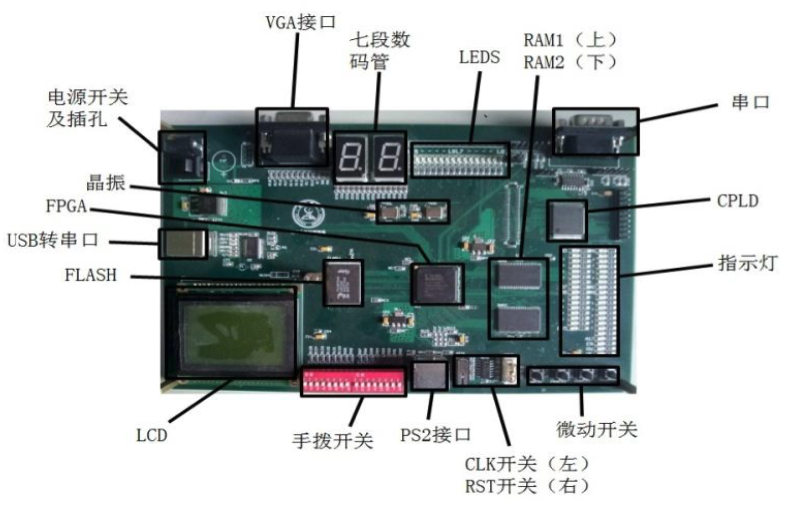
\includegraphics[width=5in]{Figures/THINPAD.png}
\end{figure}

%-----------------------------------
%	SUBSECTION 1
%-----------------------------------
\subsection{FPGA芯片}
THINPAD教学计算机上的主实验芯片是一片FPGA芯片,是由Xilinx公司生产的Spartan-3E系列的XC3S1200EFGG320芯片。FPGA芯片的具体技术参数为
\begin{center}
\footnotesize
\begin{tabular}{|c|c|c|c|c|c|c|c|}
\hline
器件名称 & 逻辑单元 & 系统门数 & CLB阵列 & CLB总数 & 用户I/O & BlockRam(Kb)\\\hline
XC3S1200E & 19512 & $1.2\times 10^6$ & $60\times 46$ & 2168 & 304 & 504\\\hline
\end{tabular}
\end{center}

FPGA管脚连接SRAM、FLASH存储器和拨码开关、LED灯、七段数码管、PS2、VGA、串口等外部设备。

%-----------------------------------
%	SUBSECTION 2
%-----------------------------------

\subsection{CPLD芯片}
THINPAD教学计算机上的扩展芯片是一片CPLD芯片,是由Xilinx公司生产的XC9500系列的XC95144XL-7TQ100芯片,它具有100个管脚、144个宏单元,采用TQFP封装。

计算机组成原理实验中,扩展CPLD充当串口控制器,完成串行数据传输的功能。CPLD配置成为一个UART(通用异步收发器),是一种广泛使用的串行数据传输装置。

%-----------------------------------
%	SUBSECTION 3
%-----------------------------------

\subsection{SRAM存储器}
THINPAD教学计算机使用了2片SRAM(Static Radom Access Memory)作为主要存储器,采用的是ISSI公司生产的异步高速CMOS SRAM,型号为IS61LV25616-10TI,每片存储容量为256K$\times$16b。

两块SRAM芯片中RAM1为基本内存,与CPLD共用基本数据总线和地址总线,RAM2为扩展内存,拥有独立的地址线和数据线。

%-----------------------------------
%	SUBSECTION 4
%-----------------------------------

\subsection{Flash存储器}
THINPAD教学计算机使用Flash存储器存储实验系统数据。使用的Flash芯片型号为MT28F640J3,数据线为16位,地址线为23位,可寻址空间8MB。Flash存储器兼具RAM和ROM的长处,不仅可以快速读取数据,也可以擦除、修改数据,同时数据不会因为断电丢失。

%-----------------------------------
%	SUBSECTION 5
%-----------------------------------

\subsection{总线}
THINPAD教学计算机上共有三条总线,分别是基本总线、扩展总线和Flash总线,它们各自分别有数据、地址和控制线。

基本总线的数据线16位、地址线18位、控制线3位。基本总线连接有多个器件,包括实验FPGA、基本内存RAM1、扩展CPLD和LED指示灯,由FPGA控制总线的访问。

扩展总线的数据线16位、地址线18位、控制线3位,连接实验FPGA和扩展内存RAM2。

Flash总线的数据线16位、地址线23位、控制线9位,连接实验FPGA和Flash存储器。

%-----------------------------------
%	SUBSECTION 6
%-----------------------------------

\subsection{外部接口}
THINPAD教学计算机硬件平台提供了一些常用外部设备的接口,包括2个七段数码管、16位LED发光二极管、拨码开关、微动开关、复位开关、一个普通串口和一个USB转串口电路、一个PS2接口用于接收键盘输入,以及一个VGA接口用于进行显示器输出。

%----------------------------------------------------------------------------------------
%	SECTION 2
%----------------------------------------------------------------------------------------

\section{软件环境}

\subsection{FPGA开发工具}
实验使用的FPGA开发工具软件为Xilinx ISE 14.7,使用的硬件开发语言为VHDL。

\subsection{THINPAD软件包}
实验使用THINPAD教学计算机软件包提供的监控程序、终端程序、Flash\& RAM读写程序、汇编程序等,并进行了相关程序的改进。

